\cotefile{103}
\scanpage{2}\mspage{1}
\margin{\handwritten{9/74\\ Envoyé par Grothendieck}}

\begin{center}
Esqu\deleted{ç}isse d'une théorie des Gr-Catégories\\
par Mme Hoang Xuan Sinh
\end{center}

Nous donnons un résumé de quelques résultats sur les (Gr)-catégories, faisant l'objet d'un travail détaillé que l'auteur compte présenter prochainement comme thèse de doctorat\handwritten{[\, ]}.

1. Structure des (Gr)-catégories.

Notre terminologie est celle de Saavedra \handwritten{[\, ]}. Nous nous intéressons à des catégories $C$ munies d'une opération binaire $(\deleted{\unsure{x|Y}}X,Y)\handwritten{\mapsto}X\otimes Y$ (fonc\deleted{\rlap{xxx}\unsure{teu|te}}teur de $C\mathbin{\mathrm{x}}C$ dans $C$) associative et unitaire à isomorphisme donné près (satisfaisant des conditions de compatibilité explicitées dans loc. cit.), appelées aussi $\otimes$-catégories AU (associatives-unitaires). On dit qu'une telle catégorie est une (Gr)-catégorie si \inserted{\handwritten{c'est un groupoïde, et si}} tout objet $X$ de $C$ est ``inversible'', i.e. admet un objet ``inverse'' $Y=X^{-1}$ (satisfaisant $X\otimes Y\handwritten{\simeq}Y\otimes X\handwritten{\simeq}1_C$, où $1_C$ désigne l'objet unité de $C$). Les exemples abondent:

\uline{Exemple\handwritten{s}\unsure{.|,}\deleted{1}} \handwritten{1.} $X$ étant un espace topologique\inserted{ ponctué par $x\handwritten{\in}X$}, on prend pour $C$ la catégorie des lace\deleted{\rlap{x}\unsure{s|t}}ts de $X$ en $x$, avec comme morphismes les classes d'homotopie d'homotopies entre lacets, comme opération $\otimes$ la composition des lacets (qui n'est pas associative, mais associative ``à homotopie près'').
% The beginnings of several lines of this left marginal note are clipped by the scan edge.
\margin{\handwritten{\figure{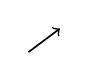
\begin{tikzpicture}[x=1cm,y=1cm]\draw[->,line width=.6pt] (0,0)--(.4,.3);\end{tikzpicture}} \unsure{Cet|cet} exemple \unsure{est|st} un cas \unsure{particulier} du \unsure{suivant}, en \unsure{prenant} $G$ $\unsure{\phantom{=}|=}\Omega^{1}(X,x)$ \unsure{(espace} des \unsure{lacets}).}}

% The recurring capital below is an overstruck typewriter glyph; its identity remains uncertain.
Variante: $\unsure{\mathbb{G}|G|E|K}$ est un espace de Hopf associatif (ou simplement homotopiquement associatif en un sens suffisamment fort), $C$ la catégorie dont les objets sont les points de $\mathbb{G}$, les morphismes les classes d'homotopies de chemins entre points de $\mathbb{G}$, la loi $\otimes$ étant induite par la loi de composition de $\mathbb{G}$. (NB Lorsque $\mathbb{G}$ admet un espace classifiant $X$, on retrouve essentiellement l'exemple précédent\handwritten{.)}\deleted{\handwritten{qui lui \unsure{même|mêmes} \illegible{2}}}

\deleted{\uline{Exemple}} 2. Si $F$ est un faisceau sur un espace topologique (ou plus généralement sur un topos), la catégorie $C$ des torseurs sous $F$, munie de la composition de Baer, est une (Gr)-catégorie (et même une catégorie de Picard stricte, cf. plus bas). On peut considérer la catégorie $C$ des Modules inversibles sur un espace (ou topos) \inserted{\handwritten{localement}} annelé \deleted{\rlap{xxxxx}comme} $(X,\underline{O}_{X})$ comme le cas particulier correspondant au cas $F=\underline{O}_{X}^{\handwritten{*}}$.

\deleted{\uline{Exemple}} 3. Si $A$ est une catégorie, la sous-catégorie pleine \inserted{\handwritten{$C$}} de $\underline{\mathrm{Hom}}(A,A)_{\handwritten{\mathrm{is}}}$ formée des équivalences de $A$ avec elle-même, munie de l\deleted{o}\handwritten{'}opération de composition des foncteurs, est une (Gr)-catégorie. Au lieu de prendre pour $A$ une catégorie, on peut \inserted{\handwritten{plus généralement}} prendre pour $A$ un objet d'une 2-catégorie quelconque. Si p.ex. $F$ est un faisceau en groupes (pas nécessairement commutatif\deleted{\unsure{s|x}}) sur un espace topologique \handwritten{(}ou un topos\handwritten{)}\deleted{$X$}\handwritten{,}
% archive sheet number: 1

\scanpage{3}\mspage{2}

prenant pour $A$ la ``champ'' sur $X$ formé des $F$-torseurs à droite, la (Gr)- catégorie des au\deleted{ot}to-équivalences de $A$ avec lui-même s'interprète comme la catégorie des ``b\deleted{t}itorseurs'' sous $F$, i.e. des faisceaux \inserted{$P$} sur lesquels $F$ opère à la fois à droite et à gauche, ces opérations commutant et chacune d'elles faisant de $P$ un torseur (à droite ou à gauche) sous $F$, - la composition $\otimes$ étant la composition de Baer évident\deleted{\unsure{e|s}}e. Lorsque $F$ est encore de la forme $\underline{O}_{X}^{*}$ ($\underline{O}_{X}$ étant un\unsure{'|.} faisceau d'anneaux, qu'on ne suppose plus nécessairement commutatif) ces bitorseurs s'interprètent aussi en termes de bi-Modules \handwritten{``}inversibles\handwritten{''} sous $\underline{O}_{X}$.

\uline{Structure}. \deleted{\rlap{xxx}\unsure{Les|les}} Soit $C$ une (Gr)-catégorie, on lui associe

a) le groupe $\handwritten{\pi}_{0}(C)$ des classes d'isomorphisme d'objets de $C$,

b) le groupe $\handwritten{\pi}_{1}(C)$ des automorphismes de $1_C$ (objet unité de $C$)

c) une action de $\handwritten{\pi}_{0}(C)$ sur $\handwritten{\pi}_{1}(C)$, en associant à tout objet $X$ de $C$ l'automorphisme \deleted{\rlap{xxxx}de 1} $\handwritten{\rho}(X)$ de $1_C$ déduit des deux isomorphismes
\diagram{\begin{tikzcd}[ampersand replacement=\&]
\mathrm{Aut}(1_C) \handwritten{\arrow[r,shift left=.55ex]\arrow[r,shift right=.55ex]} \& \mathrm{Aut}(X)
\end{tikzcd}}
donnés par $u\handwritten{\mapsto}u\otimes\mathrm{id}_{X}$ et $u\handwritten{\mapsto}\mathrm{id}_{X}\otimes u$. On prouve que $\handwritten{\pi}_{1}(C)$ est un groupe \uline{commutatif} et que l'on obtient bien par c) une structure de $\handwritten{\pi}_{0}(C)$-module sur celui-ci. Ceci posé, si on choisit pour tout $a\handwritten{\in}\handwritten{\pi}_{0}(C)$ un représentant $L_{a}\handwritten{\in}\mathrm{Ob}\ C$ de $a$, et pour deux \deleted{\rlap{xxxxxx}objets} $a,b$ un isomorphisme
\[
\handwritten{\phi}_{a,b}: L_a\otimes L_b\handwritten{\simeq}L_{ab}\ ,
\]
alors pour trois éléments $a,b,c\handwritten{\in}\handwritten{\pi}_{0}(C)$, l'isomorphisme d'associativité
\[
(L_a\otimes L_b)\otimes L_c\handwritten{\simeq}L_a\otimes(L_b\otimes L_c)\ ,
\]
compte tenu des isomorphismes $\handwritten{\phi}_{a,b}$, $\handwritten{\phi}_{ab,c}$, $\handwritten{\phi}_{b,c}$ et $\handwritten{\phi}_{a,bc}$, peut s'interpréter comme un isomorphisme
\[
L_{abc}\handwritten{\simeq}L_{abc}\ ,
\]
ou encore comme la tensorisation \deleted{\unsure{à|a}}à gauche avec un élément bien déterminé
\[
f(a,b,c)\handwritten{\in}\handwritten{\pi}_{1}(C)\deleted{\rlap{$\mathrm{xxxxxxxxx}_{\mathrm{xxxxxx}}$}\unsure{1_{C}\quad 1_{C}}}\ .
\]
Les $\handwritten{\phi}_{a,b}$ étant choisis, on voit donc que la donnée d'un isomorphisme d'associativité fonctoriel $(L\otimes L')\otimes L''\handwritten{\simeq}L\otimes(L'\otimes L'')$ équivaut à la donnée de l'application
\[
f:\handwritten{\pi}_{0}\mathbin{\mathrm{x}}\handwritten{\pi}_{0}\mathbin{\mathrm{x}}\handwritten{\pi}_{0}\handwritten{\longrightarrow}\handwritten{\pi}_{1}\ .
\]
On vérifie alors que l'axiome \deleted{\handwritten{\unsure{(du pen}}} standard d'autocompatibilité d'une donnée d'associativité \inserted{\handwritten{(axiome du pentagone)}} s'exprime précisément par la condition que $f$ soit un \handwritten{3}-\uline{cocycle} du groupe $\handwritten{\pi}_{\deleted{1}\handwritten{0}}$ à valeurs dans le groupe $\handwritten{\pi}_{1}$. D'autre part, l'indétermination dans le choix du système d'isomorphismes $\handwritten{\phi}_{a,b}$ est précisément donnée par une 2-cochaine arbitraire, et on voit que si on change $\handwritten{\phi}$ par une 2-coc\deleted{ah}haine $g$, $f$ est changé en $f+dg$ - donc l'ensemble des $f$ \deleted{p}co\deleted{\unsure{s|e|r}}rrespondants à des choix différents de $\handwritten{\phi}$ est exactement une classe de \handwritten{3}-cohomologie

% archive sheet number: 2

\scanpage{4}\mspage{3}
\[
k(C)\handwritten{\in}H^{\handwritten{3}}(\handwritten{\pi}_{0}(C),\handwritten{\unsure{K|\pi}}_{1}(C))\ .
\]
En précisant ces réflexions, on trouve que la classification, à $\otimes$-équivalence près, des (Gr)-catégories, se fait précisément en termes d\deleted{\rlap{x}\unsure{e}}'un groupe $\handwritten{\pi}_{0}$, d'un groupe commutatif $\handwritten{\pi}_{1}$ sur lequel $\handwritten{\pi}_{0}$ opère, et d'une classe de cohomologie (qui peut être prise arbitraire) dans $H^{\handwritten{3}}(\handwritten{\pi}_{0},\handwritten{\pi}_{1})$. La loi de \deleted{\rlap{xxxxx}comp} groupe du $H^{\handwritten{3}}$ admet d'ailleurs une interprétation ``géométrique'' à la Baer, en termes d'opérations sur les \handwritten{(}Gr)-catégories.

\uline{Cas particuliers}\quad Dans l'exemple 1, on \inserted{doit} retrouver bien sûr le premier invariant de Postnikoff $\handwritten{\in}H^{\handwritten{3}}(\handwritten{\pi}_{1}(X),\handwritten{\pi}_{2}(X))$, avec une interprétation ``géo\deleted{(}métrique'' nouvelle. Dans l'exemple 2, on trouve $\handwritten{\pi}_{0}=H^{1}(X,F)$, $\handwritten{\pi}_{1}=H^{0}(X,F)$\handwritten{,} et l'élément du $H^{\handwritten{3}}$ est nul (du fait qu'on a une ``catégorie de Picard stricte'', cf\inserted{\handwritten{ Deligne}} \handwritten{[\, ]}). Dans \deleted{\rlap{xxx}let} le dernier exemple, on a $\handwritten{\pi}_{0}={}$ groupe des classes d'isomorphisme d'autoéquivalences de $A$, $\handwritten{\pi}_{1}={}$ groupe des automorphismes du foncteur identique de $A$, et l'invariant $k(C)$ semble nouveau (même dans le cas où $C$ est la catégorie des biModules inversibles sous un Anneau $\underline{O}_{X}$, où $\handwritten{\pi}_{0}$ peut donc s'interpréter comme un ``groupoide de Brandt'' et $\handwritten{\pi}_{1}$ comme le groupe des ``unités centrales'' de $\underline{O}_{X}$). Signalons cependant que lorsque $A$ est la catégorie des torseurs sous un groupe (ordinaire) $F$, on trouve \deleted{\rlap{xxxxxxxxxxxxxxxxxxx}un élement de $H^{\handwritten{3}}($} $\handwritten{\pi}_{0}={}$ groupe des automorphismes extérieurs de $F$, $\handwritten{\pi}_{1}={}$ centre de $F$, et l'élément $k(C)$ du $H^{\handwritten{3}}$ n'est autre que le classique invariant de Mac-Lane. Il resterait à \deleted{\rlap{xxxxxxxx}établir}\inserted{développer} un lien \inserted{géométrique} \uline{direct} entre la théorie de\deleted{\unsure{s|x}} Mac-Lane des extensions de groupes non commutatifs\deleted{\unsure{,|s}} et des liens (``kernels''\deleted{\unsure{)|,}} dans sa terminologie) auxquels ils sont associés, et la théorie \deleted{\rlap{xxxxxxxxxxxxxxxx}développées ici,} esquissée ici des (Gr)-catég\deleted{\unsure{rr|or}}ories et de leurs splittages.

2. \uline{Catégories de Picard}.

On appelle ``catégorie de Picard'' une $\otimes$-catégorie ACU (associative-commutative-unitaire , cf. \handwritten{[\, ]}) qui est une (\deleted{E}Gr)-catégorie pour sa \deleted{\rlap{xxxx}(Gr)} $\otimes$-structure AU. On dit que c'est une catégorie de Picard \uline{stricte} si pour tout $X\handwritten{\in}\mathrm{Ob}\ C$, la symétrie de $X\otimes X$ est l'identité. Ces \deleted{\rlap{xxxxx}catég} dernières catégories sont étudiées systématiquement (dans le contexte plus général des ``champs de Picards'') par Deligne \handwritten{[\, ]}.

Soit $C$ une catégorie de Picard. En tant que (Gr)-catégorie, $C$ possède des invariants $\handwritten{\pi}_{0}$ et $\handwritten{\pi}_{1}$, mais dans le cas actuel $\handwritten{\pi}_{0}$ est aussi commutatif et agit trivialement sur $\handwritten{\pi}_{\handwritten{\unsure{0|1}}}$. On fera attention ici qu'une équivalence de (Gr)-catégories entre deux catégories de Picard $C,C'$ n'est pas nécessairement compatible avec les contraintes de commutativité, donc n'est pas nécessairement une équivalence de catégories de
% archive sheet number: 3

\scanpage{5}\mspage{4}

Picard - on peut dire que la classification ``au sens Picard'' est plus fine que la classification au sens des (Gr)-catégories. \deleted{\unsure{x}}

Associant à tout $X\handwritten{\in}\mathrm{Ob}\ C$ la symétrie de $X\otimes X$, interprété comme \deleted{\rlap{xxxx}étan} étant la tensorisation par un élément bien déterminé $s(X)$ de $\handwritten{\pi}_{1}(C)=\mathrm{Aut}(1_C)$, on trouve un\deleted{e} \deleted{\rlap{xxxxxxxxxxx}application}\inserted{homomorphisme} canonique
\[
s(C)=s:\handwritten{\pi}_{\deleted{1}\handwritten{0}}\handwritten{\longrightarrow}\unsure{{}'|\cdot}{}_{2}(\handwritten{\pi}_{\deleted{0}\handwritten{1}})\ ,
\]
où $ {}_{2}(\handwritten{\pi}_{\deleted{0}1})$ désigne le sous-groupe des éléments $x$ de $\handwritten{\pi}_{1}$ tels que $2x=0$.

Le résultat principal de la théorie de structure des catégories de Picard peut s'énoncer en disant que $C$ est déterminée (à équivalence \inserted{\handwritten{non canonique}} de catégories de Picard près) par la donnée des groupes commutatifs $\handwritten{\pi}_{0}$ et $\handwritten{\pi}_{1}$, et l'homomorphisme $s:\handwritten{\pi}_{0}\handwritten{\longrightarrow}{}_{2}(\handwritten{\pi}_{1})$. Dire que cet homomorphisme est nul signifie d'ailleurs que $C$ est une catégorie de Picard \uline{stricte}, et on retrouve le résultat de \handwritten{[\, ]} suivant lequel une catégorie de Picard stricte est déterminée (à équivalence près) par la connaissance de ses seuls invariants $\handwritten{\pi}_{0}$ et $\handwritten{\pi}_{1}$.

\uline{Remarques}. La théorie de loc. cit. nous permet, plus précisément, d'interpréter la \deleted{e}2-catégorie des catégories de \deleted{E}Picard strictes en termes de la sous-catégorie pleine de la catégorie dérivée de (Ab) (cat. des groupes abéliens), formée des complexes $K^{\deleted{\unsure{\bullet|\cdot}}}_{\handwritten{\bullet}}$ tels que $H^{\deleted{\unsure{i|1}}}_{\handwritten{i}}(K^{\deleted{\bullet}}_{\handwritten{\bullet}})=0$ pour $i\handwritten{\ne}0,1$. Le résultat précédent, assez grossier, se réduit \inserted{alors} à la remarque qu'un objet de cette catégorie est déterminé \deleted{\unsure{à|a}}à isomorphisme (non unique \handwritten{!}) près par la connaissance de son $H^{\deleted{1}}_{\handwritten{0}}$ $(=\handwritten{\pi}_{0})$ et $H^{\deleted{0}}_{\handwritten{1}}$ $(=\handwritten{\pi}_{1})$. Il y aurait lieu de développer également pour les catégories de Picard non nécessairement strictes, et pour les (Gr)-catégories, une théorie de structure pour la 2-catégorie qu'ils forment. De plus, ces \deleted{\rlap{xxxxxxxxx}résultats}\inserted{développements} encore dans les limbes, \deleted{\unsure{de|ce|co}}tout comme ceux que \deleted{\rlap{xxxxxxxxxxxxxxxxxxxxxxxx}nous avons effectivement} nous venons d'esquisser, devraient être un jour \deleted{\rlap{xxxxxxxxxx}étendus \unsure{éu|áu|au}} étudiés dans le cadre des champs (en (Gr)-catégories, ou en catégories de Picard) tout comme dans \inserted{\handwritten{Deligne}} \handwritten{[\, ]}.

\deleted{2} \handwritten{3}. \uline{Catégories de Picard enveloppantes}.

Soient $C$ une \deleted{\rlap{xx}\unsure{ca|la}} $\otimes$-catégorie AUC (par ëxemple une catégorie avec objet final et admettant des \inserted{\handwritten{\unsure{''|:}}}produits cartésiens de deux éléments), $S$ une partie de $\mathrm{Ob}\ C$. On se pose le problème universel d'envoyer (par un $\otimes$-foncteur AUC) $C$ dans une \inserted{$\otimes$-}catégorie \deleted{\unsure{$G$}}\inserted{AUC $G$}, de tel\handwritten{\unsure{é|le}} façon que pour tout $X\handwritten{\in} S$, $F(X)$ soit un objet \uline{inversible} de $G$. Le résultat principal ici est que ce problème admet toujours une solution, qu'on pourra appeler la $\otimes$-catégorie AUC ``de fractions'' par rapport à l'ensemble $S$, et noter \handwritten{\unsure{é|e}}ventuellement $S^{-1}C$. On trouve en fait que pour toute $G$, le foncteur naturel
% archive sheet number: 4

\scanpage{6}\mspage{\unsure{\phantom{5}|5}}
\[
\underline{\mathrm{Hom}}_{\otimes\mathrm{AUC}}(S^{-1}C,G)\handwritten{\longrightarrow}\underline{\mathrm{Hom}}_{\otimes\mathrm{AUC}}^{S}(C,G)
\]
(où l'exposant $S$ dans le deuxième membre dénote la sous-catégorie pleine formée des $\otimes$-foncteurs AUC $F:C\handwritten{\longrightarrow}G$ tels que $\deleted{P}F(X)$ soit inversib\unsure{\textperiodcentered|-}le pour tout $X\handwritten{\in}\mathrm{Ob}\ S$) est un \uline{isomorphisme} \uline{de catégories}.

Nous n'explicitons pas ici la construction, assez naturelle, mais dont l'explicitation pas à pas, \deleted{\rlap{xx}et}\inserted{avec} la vérification de toutes les compatibilités voulues, est fort longue et fastidieuse. Signalons seulement ici que lorsque $S$ est l'ensemble de tous les objets de $C$, $S^{-1}C$ est elle-même une catégorie de Picard (pas nécessairement stricte)\unsure{\textsuperscript{.}|'}, qu'on pourra appeler la ``catégorie de Picard enveloppante'' de $C$. C'est sans doute le cas le plus important. Les invariants $\handwritten{\pi}_{0}$ et $\handwritten{\pi}_{1}$ \deleted{\unsure{le|de}}de cette catégorie enveloppante méritent la notation $K^{0}_{\deleted{0}}(C)$ et $K^{\unsure{1|\deleted{0}1|\deleted{1}1}}_{\deleted{1}}(C)$ respectivement. Par exemple, lorsque $C$ est la catégorie des modules projectifs de type fini sur un anneau $A$, \inserted{avec l'opération de somme,} on peut démontrer que ces groupes ne sont autres que les classiques invariants $K^{0}(A)$ et $K^{1}(A)$ étudiés par Grothendieck et par Whitehead-Bass. Le même résultat est sans doute valable pour toute catégorie additive $C$ (munie de \deleted{\rlap{xx}la} l'opération somme), Cela donne une interprétation remarquable des invariants $K^{0}$ et $K^{1}$ en termes d'une ``catégorie stabilisée'' \handwritten{(}de la catégorie additive $C$\handwritten{)}, laquelle est une catégorie de Picard. Signalons seulement que, cette catégorie stabilisée (même dans le cas particulier des modules projectifs de type fini sur l'anneau $A$) n'\deleted{\unsure{est}}\handwritten{ét}ant pratiquement jamais une catégorie de Picard \uline{stricte}, ces considérations semblent rendre peu probable qu'on arrive à construire un objet canonique dans la catégorie dérivée de la catégorie (Ab), qui soit un complexe de chaines satisfaisant $H_{0}(K_{\bullet})=K^{0}$, $H_{1}(K_{\bullet})=K^{1}$ - puisqu'une telle construction (grâce à la théorie de Deligne) nous fournirait précisément une catégorie de Picard \uline{stricte} canonique dont les invariants seraient $K^{0}$ et $K^{1}$.

On peut difficilement échapper à la question d'une interpétation géométrique analogue des invariants $K^{i}$ supérieurs. Il y a tout lieu de croire qu'une telle interprétation est à\unsure{\textasciidieresis|''} chercher dans la théorie des $n$-catégories de Picard (en un sens convenable) et la construction des $n$-catégories de Picard enveloppantes d'une $\otimes$-catégorie AUC (ou d'une $\otimes$-$n$-catégorie AUC) arbitraire $C$, dont les invariants ``homotopiques'' $\handwritten{\pi}_{i}$ seraient les $K^{i}$ cherchés. De tels développeme\deleted{b}nts obligerai-
% The live text ends here on this scan with the printed continuation hyphen.

\deleted{Comme \deleted{\unsure{dans}}autre direction de recherche ouverte, suggérée par les résultats esquissés ici, signalons la construction d'une $\otimes$-catégorie de fractions d'une $\otimes$-catégorie AU (sans donnée de commutativité néces-}
% archive sheet number: 5

\scanpage{7}

ent sans doute à tirer au clair les relations très étroites qu'on pressent entre les notions de $n$-catégorie (et de $\infty$-catégorie) d'une part, celle d'ensemble simplicial (ou d'espace topologique ...) d'autre part, tout comme la relation entre $n$-Gr-catégories (et $\unsure{6\!o|\infty}$-Gr-catégories) et groupes simpliciaux (ou groupes topologiques), enfin entre \deleted{\rlap{xxxxxxxxx}la notion} \deleted{\rlap{xx}de} $n$-catégories de Picard \uline{strictes,} et \deleted{\rlap{xx}\unsure{la|le}} complexes de chaines tronqués à la dimension $n$. Il y aurait à s'attendre à une fusion \deleted{de}plus ou moins complète entre ces trois visions: algèbre homologique, algèbre \deleted{\unsure{hat|hot|hom|ham}}homótopique\margin{\unsure{*|.|\phantom{*}}}, algèbre catégorique, dans une vision comm\uline{u}ne (qui pourrait bien prendre le nom d'\handwritten{``}algèbre homologique non commutative\handwritten{''}, étant entendu que ce qui porte actuellement ce nom n'est que l'amorce de ce qui \deleted{reste à} \inserted{\handwritten{doit}} venir ...)
% The uncertain margin mark stands high beside the source line ending homóto-. Its phantom alternative records possible nontextual status; the physical mark is present.

Comme dernière question, plus terre à terre, signalons celle liée à la remarque \deleted{que} \inserted{\handwritten{suivante.}} \deleted{l}\handwritten{L}orsque \deleted{(p.ex.)} $C$ est la catégorie des modules p\deleted{or}rojectifs de type fini sur un anneau $A$ \uline{commutatif} (ou plus généralement une catégorie additive munie d'une opération $\otimes$ \deleted{\unsure{ACU|AUC}} \inserted{\handwritten{ACU}} \uline{biadditive}), alors la catégorie de Picard enveloppante, en plus de sa \deleted{str}loi de composition évidente de ``somme'' (notée ici $\oplus$ ) donnée \deleted{\rlap{xxxx}avec} \inserted{par} sa définition même, est munie d'une opération $\otimes$ provenant d\deleted{a}e l'opération de produit tensoriel \inserted{\handwritten{ordinaire}} de\handwritten{s} modules, qui en fait également une $\otimes$-catégorie ACU (mais évidemment pas une (Gr)-catégorie), liée par des isomorphismes de distributivité évident\deleted{e}\handwritten{s} \deleted{\handwritten{\unsure{aux|à}}} \deleted{\rlap{xxx}aux} \inserted{à l'}opération\deleted{s} $\oplus$. Il y aurait lieu d'étudier systématiquement les catégories $A$ ainsi munies de deux opérat\deleted{\rlap{x}a}ions $\deleted{\unsure{\otimes|\oplus}}\handwritten{\oplus}$ et $\otimes$, toutes deux AUC (des données supplémentaires), avec une donnée de distributivité
\[
X\otimes(Y\oplus Z)\handwritten{\simeq}X\otimes Y\oplus X\otimes Z
\]
et des compatibilités convenables pour celle\deleted{\unsure{s}}-ci; et de tenter de faire une théorie de structure pour de telles catégories qui sont de \deleted{\rlap{xxxxx}Picar} Picard pour la structure $\oplus$. Cela implique en particulier que $\handwritten{\pi}_{0}(A)$ est un anneau unitaire commutatif, et $\handwritten{\pi}_{1}(A)$ un module sous ce dernier. Quels autres invariants faut-il introduire pour caractériser $A$ à équivalence près respectant toutes les structures ?

% archive sheet number: 6

\scanpage{9}

\unsure{Lodève} \unsure{le} \unsure{.|,|2}7.8.74\\
Cher Deligne,\\

% Marginal note runs bottom-to-top beside the upper body; its first line is clipped at the outer edge.
% No insertion caret attaches it to a particular word of the main text.
\margin{\unsure{je n'ai pas|Je n'ai pas} \unsure{retrouvé} la \unsure{lettre} \unsure{sur les} \unsure{Gr-Champs|Gr-champs} que tu \unsure{cites|cités}}

Étant peut-être empêché par \unsure{une|ma} jambe d'assurer un cours de $1^{\mathrm{er}}$ cycl\unsure{\phantom{e}|e} au $1^{\mathrm{er}}$ trimestre, je vais peut-être \unsure{a|à|c} la place faire un petit séminaire d'algèbre, et envisage de le faire sur les fourbis de \unsure{Mme} Sinh, \unsure{éventuellement} transposés dans le contexte des ``champs''. À ce propos, je tombe sur le truc suivant, qui pour l'instant reste heuristique. Si $M,N$ sont deux faisceaux abéliens sur un topos $X$, et $\tau_{\leq 2}\mathbb{R}\unsure{{}^{\cdot}|\phantom{{}^{\cdot}}}\underline{\mathrm{Hom}}(M,N)=E(M,N)$ est le complexe ayant les invariants
% The small raised point immediately after R has uncertain textual status and attachment.
\[
\left\{\begin{aligned}
\underline{H}^{i}&=\underline{\deleted{\unsure{\mathrm{Hom}|\mathrm{Ext}}}\mathrm{E}\overset{\unsure{\cdot|\phantom{\cdot}}}{\mathrm{x}}\mathrm{t}}^{i}(M,N) &&\text{pour }0=i\leq 2\\
\underline{H}^{\unsure{j|i}}&=0 &&\text{si }i\notin[0,2]
\end{aligned}\right.
\]
% The isolated point is physically above the x region of the overwritten operator.
% Its status, attachment and possible membership in a former exponent remain uncertain.
il doit y avoir un triangle distingué canonique
\diagram{\begin{tikzcd}[ampersand replacement=\&,column sep=small]
{} \& {} \& \underline{\mathrm{Hom}}(M,{}_{2}N)[-2\unsure{\cdot|\phantom{\cdot}}]\arrow[dl] \& {}\\
(T) \& E(M,N)\arrow[rr] \& {} \& E'(M,N)\arrow[ul]
\end{tikzcd}}
% A minute isolated point just inside the closing shift bracket has uncertain textual status; the phantom alternative denotes possible nontextual status, not absence of the physical spot.

% archive sheet number: 8

\scanpage{10}

donc $E'(M,N)$ est un complexe dont les invariants $\underline{H}^{i}$ sont ceux de $E(M,N)$ en degré $i\unsure{\ne|+}2$, et qui en degré $2$ donne lieu : une suite exacte
\[
0\longrightarrow\underline{\mathrm{Ext}}^{2}(M,N)\longrightarrow
\overbrace{\underline{H}^{2}\bigl(E'(M,N)\bigr)}^{P(M,N)}
\xrightarrow{\sigma}\underline{\mathrm{Hom}}(M,{}_{2}N)\longrightarrow 0
\tag*{\makebox[0pt][r]{\makebox[\displaywidth][l]{$(*)$}}}
\]

Heuristiquement, $E'(M,\deleted{\unsure{\phantom{M}|M|N}}\unsure{N|\mathbb{N}})$ est le complexe qui exprime le ``2-champ de Picard \deleted{\unsure{``|s}}strict'' formé des 1-champs de Picard (pas nécessairement stricts) \inserted{``épi-glés'' par $M,N$} sur des objets variables de $X$, en admettant que ta théorie pour les 1-champs de Picard \inserted{stricts} s'étend aux 2-champs de Picard stricts (ce qui pour moi ne fait guère de doute) ; de même $E(M,N)$ correspond aux champs de Picard \unsure{str\uline{ict}s|st\uline{rict}s} épi-glés par $M,N$.

La suite exacte $(*)$ se construit en tous cas canoniquement ``à la main''\unsure{,|)} où $\deleted{\unsure{\mathrm{d}|\mathrm{l}}}\overset{\unsure{\cdot|\phantom{\cdot}}}{\deleted{\mathrm{e}}}$ terme médian est le faisceau des \unsure{classes|choses} \inserted{à} \deleted{\unsure{d'|à}} ``équivalence'' près des

% archive sheet number: 9

\scanpage{11}
\deleted{\unsure{catégories|catégorie}}\inserted{\unsure{champs}} de Picard \unsure{épi-glés|épinglés} par $M,N$, $\sigma$ étant l'invariant qui \inserted{s'obtient en} associant à toute section \inserted{$L$} d'un champ de Picard la symétrie de $\deleted{\unsure{K|L}}\,L\otimes L\overset{\unsure{\cdot|\phantom{\cdot}}}{,}$ interprétée comme section de ${}_{2}N$. Je sais prouver (sauf erreur) que tout hom. $M\to{}_{2}N$ provient d'un champ de Picard convenable (épinglé par $M,{}^{\unsure{\text{,}|?|\phantom{?}}}\!N$) (a priori l'obstruction est dans $\operatorname{Ext}^{3}(X;M,N)$, mais un argument ``universel'' prouve qu'elle est nulle). Cela prouve que l'extension $\alpha$, est bien proche d'être splittée :\deleted{\unsure{u|un}} tte section du troisième faisceau, sur un objet quelconque de $X$, se remonte - en d'autres termes l'extension a une section ``ensembliste''. Bien sûr, il y a mieux en fait : toute section sur un $U\in\operatorname{Ob}X$ ``provient'' d'un élément de ${\unsure{\mathcal H|\mathscr H}}^{2}(U,E'(M,N))\overset{\unsure{\cdot|\phantom{\cdot}}}{\unsure{,|\phantom{,}}}$ (hypercohomologie $\mathcal H^{2}$).
% archive sheet number: 10

\scanpage{12}

\uline{Exemple} Soit $A$ un anneau sur $X$, soient $M,N$ respectivement les faisceaux $K^{0}$ et $K^{1}$ associés au champ additif des $A$-Modules projectifs de $\mathrm{v}.\mathrm{f}\unsure{.|\phantom{.}}$ \inserted{(p\textsuperscript{r} ex.)} Alors la construction de Mme Sinh nous fournit un champ de Picard épinglé par $M,N$, d'où une section \deleted{\unsure{du|de}} canonique du terme médian $\unsure{P|F}(M,N)$ de $(\alpha)$.\unsure{'|\textsuperscript{.}|\phantom{'}}

\uline{NB} Tout ce qui précède a les fonctorialités évidentes en $M,N,X$\ldots

\uline{Question} : Le triangle exact $(\unsure{T|J})$ et - la suite exacte $\alpha)$ sont ils connus par les compétences (Quillen, Breen, Illusie\ldots) ? \deleted{\unsure{S|X}}Connaissent-ils des variantes ``supérieures'' ? (Un principe ``géométrique'' pour en obtenir pourrait être via des $n$-champs de Picard non néc. stricts\ldots)
% archive sheet number: 11

\scanpage{13}

Je profite de l'occasion pour soulever une question sur la ``cohomologie relative''. Soit $\unsure{q|g}:X\to Y$ un morphisme de topos. Si $F$ est un faisceau abélien (ou un complexe d'iceux) sur $Y$, peut-on définir \unsure{fon\uline{ctoriellem}ent|fo\uline{nctoriellem}ent} en $F$ la cohomologie relative $\mathbb R\Gamma(Y\mathbin{\mathrm{mod}}X,F)$ (de la catégorie dérivée de $\unsure{\mathbb{A}b|\mathit{Ab}}(Y)$ dans celle de $\mathbb{A}b$) ? L'interprétation ``géométrique'' en termes d'opérations sur des $n$-champs de Picard ($n$ ``grand'') suggère que ça doit exister
Mais je ne vois de construction \unsure{évident|évidente} ``\unsure{\textsuperscript{.}|\phantom{\textsuperscript{.}}}à la main'' que dans les deux cas extrêmes :

a) $q$ est ``$(-1)$-acyclique'' i.e. pour tt $F$ sur $Y$, $F\mathord{-}q_{*}q^{*}F$ est injectif (\uline{NB} c'est le cas de $Y_{/\unsure{p|P}}\to Y$ \unsure{si|où} $p\to e_{Y}$ est un \unsure{épimorphisme} - c'est donc le cas de $B_{\unsure{c|e}}\to B_{\unsure{c|G}}$ plus haut)

On prend
% isolated point at source (74,1603), left of display
\margin{\unsure{.|\phantom{.}}}
\[
\mathbb R\Gamma_{\deleted{\unsure{Y|X}}}\bigl(\operatorname{Coker}\bigl(F\to q_{*}\unsure{[|(}\underbrace{e(q^{*}(F)}_{\text{résol. inj.}}))\bigr)[-1]\bigr)
\]
% isolated point at source (202,1634), above-right of archive number
\margin{\unsure{.|\phantom{.}}}
% archive sheet number: 12

\scanpage{14}

% Wholly handwritten page: the main hand is unnamed.
% The following clipped left-edge traces have no secure lexical identification.
% Their textual status is uncertain; the phantom alternatives do not deny the ink.
\reversemarginpar
\margin{\figure{\unsure{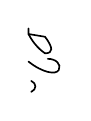
\begin{tikzpicture}[x=.35mm,y=.35mm,line width=.6pt,line cap=round]
\draw (0,16) -- (0,14) -- (6,13) .. controls (9,9) and (9,7) .. (6,7)
 .. controls (3,9) and (1,12) .. (0,14);
\draw (0,4) .. controls (5,0) and (10,-1) .. (11,1)
 .. controls (12,3) and (10,5) .. (7,5);
\draw (1,-3) .. controls (3,-4) and (3,-6) .. (1,-7);
\end{tikzpicture}|\phantom{\rule{4mm}{9mm}}}}}
\normalmarginpar
b) $\forall\,F$ injectif sur $\unsure{Y}$, $\unsure{q|g}^{*}(F)$ est injectif et $F\unsure{\mathord{-}|\to}q_{*}q^{*}F$ est un épimorphisme (ex: $q$ inclusion d'un ouvert $U\hookrightarrow e_{Y}$).
On prend
\[
\mathbb R\Gamma_{Y}\bigl(\operatorname{Ker}\bigl(\underbrace{C(F}_{\text{rés. inj.}})\to
q_{*}q^{*}\unsure{(|C}C(F)\bigr)\bigr)\bigr)
\]
% Small detached right-margin trace beside/below the first display; status uncertain.
\margin{\figure{\unsure{\begin{tikzpicture}[x=.35mm,y=.35mm,line width=.35pt,line cap=round]
\draw[gray] (0,5) .. controls (1,4) and (2,5) .. (3,5);
\fill (2,2.5) circle (.35);
\draw[gray] (2,2.2) -- (1.5,.5);
\fill[gray] (1,-1) ellipse (.3 and .65);
\end{tikzpicture}|\phantom{\rule{2mm}{4mm}}}}}

Dans le cas général, la difficulté provient du fait que le cône d'un morphisme de complexes (tel que
% Clipped left-edge upright, lower bar and point; no secure textual identity.
\reversemarginpar
\margin{\figure{\unsure{\begin{tikzpicture}[x=.35mm,y=.35mm,line width=.6pt,line cap=round]
\draw (0,8) -- (0,2);
\draw (0,0) -- (5,.4);
\fill (0,-5) ellipse (.45 and .7);
\end{tikzpicture}|\phantom{\rule{3mm}{6mm}}}}}
\normalmarginpar
\[
F\to q_{*}\deleted{\unsure{C|(}}\bigl(q^{*}(F)\deleted{\unsure{)|C}}\bigr)
\deleted{\unsure{*|q_{*}}}\qquad\text{)}
\]
n'est pas fonctoriel (dans la
% Detached dark left-edge point, textual status uncertain.
\reversemarginpar
\margin{$\unsure{\cdot|\phantom{\cdot}}$}
\normalmarginpar
catégorie dérivée) p. r. à la flèche dont on veut prendre le cône.
% Detached left-margin point near source y=914; textual status uncertain.
\reversemarginpar
\margin{$\unsure{\cdot|\phantom{\cdot}}$}
\normalmarginpar

% Clipped curved trace at the left edge beside this paragraph.
\reversemarginpar
\margin{\figure{\unsure{\begin{tikzpicture}[x=.4mm,y=.4mm,line width=.6pt,line cap=round]
\draw (0,3) .. controls (4,1) and (4,-2) .. (0,-3);
\end{tikzpicture}|\phantom{\rule{2mm}{3mm}}}}}
\normalmarginpar
Et pourtant, dans le cas particulier actuel\unsure{\phantom{,}|,} il devrait y avoir un choix fonctoriel.
% The detached point lies below-left of the hyphen between t and ce.
ESt$\underset{\hspace{-.35em}\unsure{\cdot|\phantom{\cdot}}}{\text{-}}$ce
\unsure{\.{e}vident|évident|evident} ?
\textsuperscript{\unsure{'|\phantom{'}}}
% A further clipped curved trace lies at the left edge beside the preceding question.
\reversemarginpar
\margin{\figure{\unsure{\begin{tikzpicture}[x=.4mm,y=.4mm,line width=.6pt,line cap=round]
\draw (0,3) .. controls (3,1) and (3,-2) .. (0,-3);
\fill (0,-9) ellipse (.25 and .4);
\end{tikzpicture}|\phantom{\rule{2mm}{5mm}}}}}
\normalmarginpar

% Isolated point in the gap above the rubric, source (510,1240).
\noindent\hspace{.43\linewidth}$\unsure{\cdot|\phantom{\cdot}}$\par
% Two small boundary shapes beside the rubric underline; pen origin uncertain.
\reversemarginpar
\margin{\figure{\unsure{\begin{tikzpicture}[x=.4mm,y=-.4mm,line width=.5pt,line cap=round]
\draw (0,0)--(2,1.2);
\fill (1,12) circle (.8);
\end{tikzpicture}|\phantom{\rule{2mm}{6mm}}}}}
\normalmarginpar
\unsure{Q\uline{uestion pour Illusi}e|Q\uline{uestion pour Illusie}} : Dans sa \unsure{th\.{e}orie|théorie|theorie} des déform.tions de schémas en \unsure{groupes|groupe}
% Clipped left-edge thick curved trace and small lower point.
\reversemarginpar
\margin{\figure{\unsure{\begin{tikzpicture}[x=.4mm,y=.4mm,line width=.8pt,line cap=round]
\draw (0,3) .. controls (2,1) and (2,0) .. (0,-1);
\fill (0,-6) ellipse (.25 and .4);
\end{tikzpicture}|\phantom{\rule{2mm}{4mm}}}}}
\normalmarginpar
plats, il tombe sur des $H^{3}(B_{\unsure{G|C}}/X,\quad)$ resp. des $\operatorname{Ext}^{2}(\unsure{K|X};,\quad)$.
Peut-on courtcircuiter sa théorie via la théorie (supposée écrite) des Gr-champs - resp. via la théorie des champs de Picard ? J'ai

% Two detached bottom points, below the faint horizontal paper/image rule.
\begin{center}
$\unsure{\bullet\,\cdot|\phantom{\bullet\,\cdot}}$
\end{center}
% The faint horizontal gray rule near the foot is not assigned a textual function.
% archive sheet number: 13
